\documentclass[../main.tex]{subfiles}
\usepackage{tikz}
\usepackage{xcolor}
\begin{document}

This chapter presents the background knowledge for the thesis research, including OT, ICS, PLCs, the Purdue network architecture model, the Siemens S7comm protocol, and IDS. This chapter is the basis for understanding the operating context, security weaknesses, and the approach to detecting attacks on S7comm in the following chapters.

\section{Overview of OT and ICS systems}
\label{sec:ot-ics}

All technologies used to run a physical plant are called OT, including:

\begin{itemize}
    \item Supporting monitoring and management technologies such as BMS for HVAC, lighting, and fire protection; EMS for energy consumption management.
    \item Maintenance technologies such as EAM for tracking equipment condition.
    \item Field communication and operation control technologies.
    \item ICS control technology for monitoring and controlling industrial processes. An ICS includes the following main components:
\end{itemize}

\begin{center}
    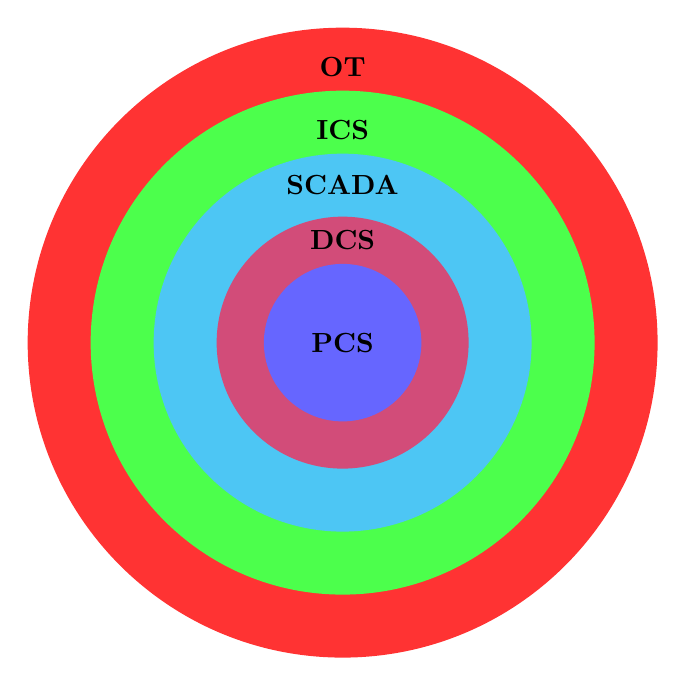
\begin{tikzpicture}
    
    % Outermost ring (OT)
    \fill[red!80] (0,0) circle (4);
    
    % ICS
    \fill[green!70] (0,0) circle (3.2);
    
    % SCADA
    \fill[cyan!70] (0,0) circle (2.4);
    
    % DCS
    \fill[purple!70] (0,0) circle (1.6);
    
    % PCS
    \fill[blue!60] (0,0) circle (1);
    
    % Text labels
    \node at (0,3.5) {\textbf{OT}};
    \node at (0,2.7) {\textbf{ICS}};
    \node at (0,2.0) {\textbf{SCADA}};
    \node at (0,1.3) {\textbf{DCS}};
    \node at (0,0) {\textbf{PCS}};
    
    \end{tikzpicture}
    \end{center}

\begin{itemize}
    \item \textbf{ICS}: controls industrial processes in general.
    \item \textbf{SCADA}: provides real-time monitoring, analysis, and high-level management for devices spread across \textbf{multiple geographic areas} from a single command center.
    
    Figure~\ref{fig:scada} shows example of a SCADA system.

\begin{figure}[H]
    \centering
    
\includegraphics[width=0.4\textwidth]{Figure/SCADA.png}
    \caption{Example of a SCADA system}
    \label{fig:scada}
    \end{figure}


    The SCADA system manages and monitors three plants in three different geographic areas: Texas, North Dakota, and Alaska. The SCADA Control Center includes Control Servers, HMI, Historian, Engineering Workstation, and Communication Infrastructure, located in the Supervisory Zone.

    \item \textbf{DCS}: focuses on controlling complex, continuous industrial processes that need coordination of many individual controllers connected through a central controller. Splitting into individual controllers for each specific process in the overall process places controllers closer to the process they control, simplifies logic, reduces delay, and eases maintenance. However, these controllers are all in the same geographic area. DCS is often used in large, complex plants where thousands of parameters must be coordinated and controlled at the same time with high reliability.

    \item \textbf{PCS}: a general term for a subsystem that performs one specific task/function in the overall production process. One ICS can include hundreds of PCS.

    Figure~\ref{fig:dcs} shows example of a DCS deployed at a plant.

\begin{figure}[H]
    \centering
    
\includegraphics[width=0.4\textwidth]{Figure/DCS.png}
    \caption{Example of a DCS deployed at a plant}
    \label{fig:dcs}
    \end{figure}

    The plant in Alaska (one of the three plants monitored by the SCADA system above) uses DCS, including many individual controllers (Local Control Unit). Each controller performs one specific function in the production line (PCS). A PCS includes the following components:

    \begin{itemize}
        \item \textbf{Field Devices}: convert between physical process signals and electronic signals, including:
        \begin{itemize}
            \item \textbf{Sensors}: measure physical parameters such as temperature, pressure, flow, humidity\ldots\ and convert them to input electronic signals.
            \item \textbf{Actuators}: receive output electronic signals to control physical equipment such as valves, pumps, motors\ldots
        \end{itemize}

        \item \textbf{Field Controller}: field controller, including:
        \begin{itemize}
            \item \textbf{PLC}: a programmable device; receives input signals $\rightarrow$ processes pre-programmed logic operations $\rightarrow$ outputs signals. It also sends process data to the HMI and receives control commands from the HMI.

            \item \textbf{IED}: similar to a PLC but specialized for electrical equipment such as protection relays, \textit{on-load tap changer}, and \textit{circuit breaker}. IEDs usually run pre-programmed programs independently rather than receiving direct control commands from the HMI.

            \item \textbf{RTU}: similar to a PLC but focused on sending \textit{telemetry} data from remote sites to the control center; often has stronger long-range communication such as RF, satellite, cellular\ldots

            \item \textbf{PAC}: extends PLC capability, close to a PC combined with a PLC; supports programming in five IEC~61131-3 languages plus C/C++. PAC supports more I/O modules, more complex logic, data processing and database integration, often used for multi-domain control and monitoring.
        \end{itemize}

        \item \textbf{HMI}: interface between humans and machines. Human $\rightarrow$ Machine converts operator actions into signals the machine understands; Machine $\rightarrow$ Human converts signals into symbols and graphs such as \textit{status}, \textit{alarms}, and \textit{notifications}.
    \end{itemize}

    \item \textbf{SIS}: a control system similar to a PLC but deployed \textbf{independently and separately} from the main control system to add an extra safety layer when the main control system fails.

    Figure~\ref{fig:sis} shows example of a SIS system.

\begin{figure}[H]
    \centering
    
\includegraphics[width=0.4\textwidth]{Figure/SIS.png}
    \caption{Example of a SIS system}
    \label{fig:sis}
    \end{figure}

    The SIS Controller is also like a PLC/RTU but uses its own 2 Level Gauges sensors and 2 Valve Actuators to control water level in the tank. Even if the PLC fails or the main sensor has problems, the backup SIS still ensures safety.

    \item \textbf{EMS}: energy management system that helps optimize use, transmission, and distribution of energy so the plant runs efficiently and does not overload the power grid.
\end{itemize}

\section{PLC}
\label{sec:plc}

\subsection{PLC concept}

A PLC is a programmable logic controller. In essence, a PLC is like a PC running a program written by a programmer. The only difference is hardware quality: it is especially robust and compact so it can withstand the harsh environment of manufacturing plants---vibration, high temperature, dust, electromagnetic interference, and continuous 24/7 operation for many years.

Before PLCs existed, control of these processes was usually done with hundreds or even thousands of electromechanical relays, timers, and counters. Such systems were bulky, complex, and hard to change. The PLC, introduced in the late 1960s by \textbf{Richard E. Morley}, was a revolution that fully replaced traditional relay control systems. Unlike hard-wired relay control, PLC control logic can be changed easily by modifying the software program without changing hardware or rewiring.


\subsection{PLC structure}

Figure~\ref{fig:plc-components} shows main components of a PLC.

\begin{figure}[H]
    \centering
    
\includegraphics[width=0.58\textwidth]{Figure/PLC_components.png}
    \caption{Main components of a PLC}
    \label{fig:plc-components}
\end{figure}

\subsubsection{CPU}

The \textbf{CPU} is considered the brain of the PLC. Unlike a typical PC CPU that runs multitasking and is \textit{event-driven}, the PLC CPU runs on a \textit{scan cycle} (usually measured in milliseconds) and executes program instructions in sequence. A typical scan cycle has three main steps:

\begin{enumerate}
    \item \textbf{Input Scan}: The CPU reads sensor and button states on input modules and copies data into the \textit{Input Image Table} (PII), giving the CPU a consistent snapshot of inputs.
    \item \textbf{Program Execution}: The CPU runs the loaded program to process logic, arithmetic, and control instructions based on the inputs received.
    \item \textbf{Output Scan}: After computation, the CPU updates the \textit{Output Image Table} (PIQ), then writes to output modules to control actuators (motors, valves, lights\ldots).
    \item \textbf{Repeat the scan cycle}.
\end{enumerate}

Besides main logic execution, the CPU also handles diagnostics and communication with other PLCs or systems. PLC CPUs are usually based on Intel X86, PowerPC, ARM, or MIPS architectures.


\subsubsection{Input and output modules}

\textbf{Input Modules} receive signals from field devices and convert them into logic signals the CPU can understand. There are two main types:
\begin{itemize}
    \item Digital input module (DI -- \textit{Digital Input Module}): receives ON/OFF signals.
    \item Analog input module (AI -- \textit{Analog Input Module}): receives continuous signals.
\end{itemize}


\textbf{Output Modules} receive commands from the CPU and convert them into control signals for actuators. Similarly:

\begin{itemize}
    \item Digital output module (DO) outputs ON/OFF signals (Relay, Transistor, Triac)
    \item Analog output module (AO) outputs continuous signals.
\end{itemize} 


\subsubsection{Memory}

A PLC includes the following types of memory:

\begin{itemize}
    \item \textbf{Read-only Memory (ROM)}: Stores PLC firmware and OS. Because this part does not change during PLC operation, it is read-only. The PLC OS is usually separate and optimized for real-time environments (RTOS -- Real-time Operating System), such as VxWorks, Windows CE, Neutrino \& RTOS.
    \item \textbf{Random Access Memory (RAM)}: Stores temporary data such as I/O states, timers, counters, and internal variables. Data is lost when power is lost. Important memory areas~\cite{snap7_sharp7}:

    \begin{table}[H]
        \centering
        \caption{RAM memory areas in a PLC (Siemens notation)}
        \label{tab:plc-memory}
        \begin{tabular}{|l|c|p{7.5cm}|}
            \hline
            \textbf{Memory area} & \textbf{Symbol} & \textbf{Meaning} \\
            \hline
            Input & I or E & Stores the state of physical input ports (buttons, limit switches). The PLC reads from hardware and copies here at the start of the scan cycle. \\
            \hline
            Output & Q or A & Stores the desired state of actuators (motors, lights, valves). At the end of the scan cycle, data from here is pushed to hardware. \\
            \hline
            Memory/Merker & M & Global intermediate memory of the PLC, similar to global variables in IT. It stores intermediate algorithm states without direct output to hardware. \\
            \hline
            Data Block & DB & User data block; stores setpoints, temperature/pressure limits, passwords\ldots \\
            \hline
            Local data & L & Stores local variables in program blocks \\
            \hline
            Timer & T or \%T & Timer. \\
            \hline
            Counter & C or \%C & Event counter. \\
            \hline
        \end{tabular}
    \end{table}


    \item \textbf{Electrically Erasable Programmable Read-Only Memory (EEPROM)}: Operates on data at byte level. Data is not lost when power is lost. Usually used to store the PLC program and configuration data.
    \item \textbf{Flash Memory}: Similar to EEPROM but operates on data at block level. Larger capacity, faster, and cheaper.
\end{itemize}

\subsubsection{Other components}

The \textbf{Power Supply Unit} provides stable voltage to PLC components, with backup power (UPS) to protect devices during sudden power loss.

The \textbf{CP} lets the PLC communicate with programming workstations, HMI, SCADA, other PLCs, or data management systems. The PLC can
communicate over legacy serial links such as RS-232, RS-485 or modern RJ45 Ethernet ports.


These components can be split into separate physical modules and connected via a system bus (\textit{Modular PLC}) (Modular PLC) or integrated in a single unit (\textit{Compact PLC} or \textit{Brick PLC}).

Figure~\ref{fig:plc-types} shows siemens LOGO! --- Compact PLC.

\begin{figure}[htbp]
    \centering
    \begin{subfigure}[t]{0.45\textwidth}
        \centering
        
\includegraphics[width=\textwidth]{Figure/Compact_PLC_type.png}
        \caption{Siemens LOGO! --- Compact PLC}
    \end{subfigure}
    \hfill
    \begin{subfigure}[t]{0.45\textwidth}
        \centering
        
\includegraphics[width=\textwidth]{Figure/Modular_PLC_type.png}
        \caption{Siemens S7-1200 --- Modular PLC}
    \end{subfigure}
    \caption{Two PLC form factors: Compact and Modular}
    \label{fig:plc-types}
\end{figure}

For modular PLCs, components are mounted in \textit{slots} on the electrical cabinet \textit{rack}:

Figure~\ref{fig:plc-rack} shows in TIA Portal programming software, you must specify the rack and slot of the PLC communication module; for example, in the figure rack 0, slot 1 is needed to connect to the correct PLC.

\begin{figure}[htbp]
    \centering
    
\includegraphics[width=0.58\textwidth]{Figure/PLC_rack.png}
    \caption{In TIA Portal programming software, you must specify the rack and slot of the PLC communication module; for example, in the figure rack 0, slot 1 is needed to connect to the correct PLC}
    \label{fig:plc-rack}
\end{figure}

\subsection{PLC programming languages}

PLC control programs are written in five programming languages according to \textbf{IEC 61131-3}:

Figure~\ref{fig:plc-languages} shows five PLC programming languages per IEC 61131-3.

\begin{figure}[htbp]
    \centering
    
\includegraphics[width=0.58\textwidth]{Figure/Code_PLC.png}
    \caption{Five PLC programming languages per IEC 61131-3}
    \label{fig:plc-languages}
\end{figure}

\begin{enumerate}
    \item \textbf{Ladder Diagram (LD)}: a graphical relay-circuit language with two vertical bars (Bus Bar) representing hot and 
    neutral wires; horizontal rungs between the two bars represent control logic lines including inputs, 
    logic operations connected to outputs, contacts, and coils. The PLC scans rungs from top to bottom, 
    and each rung is scanned left to right. Each scan cycle is about 50--60~ms. This is the most popular language among PLC programmers because its 
    design thinking is similar to electronic circuit diagrams.
    
    Figure~\ref{fig:ld-example} shows example of a self-holding circuit program in Ladder language.

\begin{figure}[H]
        \centering
        
\includegraphics[width=0.48\textwidth]{Figure/Ladder.png}
        \caption{Example of a self-holding circuit program in Ladder language}
        \label{fig:ld-example}
    \end{figure}

    \item \textbf{Function Block Diagram (FBD)}: logic using function blocks. Rectangular blocks with inputs on the left and outputs on the right, connected by lines (signal wires). Allows building complex control applications visually. 

    Figure~\ref{fig:fbd-example} shows example FBD program.

\begin{figure}[htbp]
        \centering
        
\includegraphics[width=0.60\textwidth]{Figure/FBD_code.png}
        \caption{Example FBD program}
        \label{fig:fbd-example}
    \end{figure}

    \item \textbf{Sequential Function Chart (SFC)}: like a flowchart with steps and transition conditions. Used for complex sequential processes

    Figure~\ref{fig:sfc-example} shows example SFC program.

\begin{figure}[htbp]
        \centering
        
\includegraphics[width=0.60\textwidth]{Figure/SFC_code.png}
        \caption{Example SFC program}
        \label{fig:sfc-example}
    \end{figure}

    \item \textbf{Structured Text (ST)}: plain text code, similar to C / Pascal. Suitable for programmers coding complex applications with many calculations and data processing, using structures such as \texttt{IF...THEN}, \texttt{FOR}, \texttt{WHILE}

\begin{quote}
\small\ttfamily
IF Input1 THEN\\
\quad Output1 := NOT Output1;\\
END\_IF;
\end{quote}

    \item \textbf{Instruction List (IL)}: a low-level language similar to Assembly. It is a vertical list of abbreviated instructions. Requires deep knowledge of PLCs and computer architecture; used for applications needing high processing speed and performance. However, manufacturers no longer encourage its use.

\end{enumerate}

\section{Purdue model}
\label{sec:purdue}

The Purdue model (\textit{Purdue Enterprise Reference Architecture} -- PERA) is 
the standard model for dividing network layers in ICS/OT environments.

Figure~\ref{fig:purdue-overview} shows purdue network segmentation model.

\begin{figure}[H]
    \centering
    
\includegraphics[width=0.58\textwidth]{Figure/Purdue.png}
    \caption{Purdue network segmentation model}
    \label{fig:purdue-overview}
\end{figure}

This architecture shows the concept of network segmentation that separates the ICS (OT) network zone from the enterprise IT network zone. It also shows the interdependence and interaction of main components at levels 0 to 5. This model is applied in IEC 62443, a standard for cybersecurity in industrial networks.

Table~\ref{tab:purdue-layers} describes each layer and typical devices in detail.

\begin{table}[H]
    \centering
    \caption{Purdue network layers (levels 0--5)}
    \label{tab:purdue-layers}
    \footnotesize
    \renewcommand{\arraystretch}{1.25}
    \begin{tabular}{|>{\raggedright\arraybackslash}p{2.1cm}|>{\raggedright\arraybackslash}p{4.3cm}|>{\raggedright\arraybackslash}p{7.2cm}|}
        \hline
        \textbf{Layer} & \textbf{Description} & \textbf{Devices} \\
        \hline
        0 --- \textit{Physical Layer} &
        Where electrical/optical signals are converted into the physical process (with Actuator) or in the reverse direction (with Sensor). &
        \textbf{Sensor}: measures physical parameters such as temperature, images\ldots
        \par\vspace{0.3em}
        \textbf{Actuator}: valves, robot arms\ldots
        \par\vspace{0.3em}
        
\includegraphics[width=0.6\linewidth]{Figure/ABB.png} \\
        \hline
        1 --- \textit{Controller Layer} &
        Contains controllers that receive signals from Sensor $\rightarrow$ process control logic $\rightarrow$ output control signals to Actuator. &
        PLC, RTU. The PLCs themselves do not directly control robot arms; they send down a task that is only a sequence number to the robot controller. These controllers contain the actual robot control commands and execute the program corresponding to the task assigned by the PLC.
        \par\vspace{0.3em}
        
\includegraphics[width=0.6\linewidth]{Figure/PLCS7-1500.png} \\
        \hline
        2 --- \textit{Supervisor Layer} &
        Contains local monitoring equipment for \textbf{one shop} in the plant. &
        Local HMI, local PC, shop Engineering Workstation. Each PCS often has one (or several) HMIs for operators; naming often follows the pattern line + station + sequence number.
        \par\vspace{0.3em}
        
\includegraphics[width=0.6\linewidth]{Figure/HMI.png} \\
        \hline
        3 --- \textit{Operation Layer} &
        Contains monitoring and coordination equipment for \textbf{all shops}, located at the plant central control room. &
        Database, SCADA Control Center, MES is the system that coordinates production activities such as scheduling, order tracking, QC product quality monitoring. \\
        \hline
        3.5 --- \textit{DMZ Layer} &
        The DMZ layer is a buffer zone between OT and IT networks. This zone controls access through firewalls and does not allow traffic to flow directly between OT and IT. &
        Firewall, data diodes, Jump Server: machine from IT -> Jump Server (DMZ) -> machine in OT, Replica Historian: IT machines get historical data here instead of reaching into OT machines, Patch Server: because the OT network is not allowed to connect to the Internet, updates must be downloaded from Internet -> Patch Server (DMZ) -> OT machines get updates from this Patch Server (DMZ) instead of directly from the Internet. \\
        \hline
        4 --- \textit{Management Layer} &
        Internal IT network of the plant. &
        Office workstations at the central control room. ERP is the system that manages all enterprise activities, including not only plant production (MES) but also HR, finance, and supply chain. CRM. \\
        \hline
        5 &
        DMZ between internal IT network and the Internet. Connects the plant to the Internet and allows managing a plant from another geographic location. &
        Firewalls and servers exposed to the Internet such as Web Server, Email Server\ldots \\
        \hline
    \end{tabular}
\end{table}

\section{Siemens S7comm protocol}
\label{sec:s7comm}

\subsection{Background: Fieldbus and industrial Ethernet}

\textbf{Fieldbus} is an industrial network used to connect PLCs to field devices (sensor, actuator) or between PLCs or with other industrial devices. Each fieldbus standard defines:

\begin{itemize}
    \item cable type
    \item signal transmission method
    \item data transmission protocol
    \item network organization
\end{itemize}

Some common Fieldbus types:


\begin{table}[H]
    \centering
    \caption{Some common Fieldbus standards}
    \label{tab:fieldbus}
    \footnotesize
    \begin{tabular}{|l|l|l|l|}
        \hline
        \textbf{Name} & \textbf{Cable} & \textbf{Topology} & \textbf{Protocol} \\
        \hline
        PROFIBUS & RS-485 & bus & PROFIBUS \\
        \hline
        Modbus RTU & RS-485 & bus & Modbus \\
        \hline
        CAN bus & twisted pair & bus & CANopen, DeviceNet \\
        \hline
    \end{tabular}
\end{table}

\textbf{Industrial Ethernet} is another type of industrial network that uses standard Ethernet cables. Common protocols running on industrial Ethernet include: EtherNet/IP, Modbus TCP, \textbf{PROFINET}, and \textbf{Siemens S7}. 

Advantages of industrial Ethernet networks are

\begin{itemize}
    \item High speed, better compatibility with IT devices, easy to debug
    \item Lower cost than traditional fieldbus types because it uses standard Ethernet infrastructure and does not require dedicated adapters or connection cables
\end{itemize}

Siemens PLCs can communicate over Ethernet using one of the following two protocols ~\cite{snap7_s7protocol}:

\begin{itemize}
    \item \textbf{Open TCP/IP}: implements the standard TCP/IP stack, meaning the PLC uses normal TCP/IP. In this case, programs can be implemented like regular network programming using sockets, TCP, and UDP. However, this protocol only transmits data as a stream (stream-based), while Siemens control commands require fixed length (Data Block), so in PLC FC (Function Code) and FB (Function Block) programs the programmer must packetize messages from the stream data into blocks.

    \item \textbf{S7}, \textbf{S7comm}, or \textbf{S7 Communication}, with a later upgrade called \textbf{S7 comm plus}. This is a proprietary Siemens protocol that first appeared in 1994 together with the Simatic S7-200, S7-300, and S7-400 product lines. In industrial network architecture, the S7 protocol operates in a \textit{request--response} model: one side sends a request and the other replies.
\end{itemize}

\textit{Some documents use other names such as the client-server model (with S7 running on modern Ethernet with network infrastructure using full-duplex switches) or master-slave (with S7 running on older Fieldbus networks such as PROFIBUS where the network infrastructure is a single shared bus). Whatever the name, S7 still follows the request-response communication model, meaning one side sends a request and the other replies ~\cite{inprotech_s7comm_security}.}

S7 is a layer 7 protocol. However, it extends down to lower layers by reusing protocols at those layers. This is because S7 was not originally designed to run on the TCP/IP network architecture. S7 was originally designed to run on Fieldbus network infrastructure such as PROFIBUS or MPI~\cite{veit2021ics_dissectors} using dedicated industrial cables instead of Ethernet cables for transmission. 

Figure~\ref{fig:s7-network-stack} shows S7 network architecture.

\begin{figure}[H]
    \centering
    
\includegraphics[width=0.63\textwidth]{Figure/S7_stack.png}
    \caption{S7 network architecture}
    \label{fig:s7-network-stack}
\end{figure}

However, to improve compatibility, S7 Comm was enhanced to run on ISO TCP (per RFC 1006 standard), and this ISO TCP protocol in turn runs on TCP/IP. In its original design, the ISO TCP model is a packet-based or block-oriented protocol, meaning each message has a clear length. Each block is called a \textbf{PDU}. PDU length depends on the CP inside the PLC and is negotiated between devices when establishing a connection.

\subsection{How to read addresses in Siemens S7}

General syntax:

Figure~\ref{fig:s7-address} shows address syntax in Siemens S7.

\begin{figure}[H]
    \centering
    
\includegraphics[width=0.63\textwidth]{Figure/read_memory.png}
    \caption{Address syntax in Siemens S7}
    \label{fig:s7-address}
\end{figure}


Where: 
\begin{itemize}
    \item Memory area type: I (Input), Q (Output), M (Memory/Merker), DB, T (Timer), C (Counter)
    \item Size: X (bit), B (byte), W (word), D (dword)
    
    \begin{table}[H]
        \centering
        \caption{Data size notation in S7}
        \label{tab:s7-data-size}
        \footnotesize
        \begin{tabular}{|c|l|c|l|}
            \hline
            \textbf{Notation} & \textbf{Name} & \textbf{Bits} & \textbf{Example} \\
            \hline
            X & Bit & 1 & M0.3 (Merker byte 0, bit 3) \\
            \hline
            B & Byte & 8 & MB5 \\
            \hline
            W & Word & 16 & MW10 \\
            \hline
            D & DWord & 32 & MD20 \\
            \hline
        \end{tabular}
    \end{table}
    
\end{itemize}


The DB memory area has special syntax: \textit{[Memory area type]} includes \textit{DB} + the DB index, for example \textit{DB1}, \textit{DB2}; \textit{[Data size]} always has the \textit{DB} prefix instead of only the data type, for example \textit{DBW} to read a Word instead of writing only \textit{W}.

Examples: 

\begin{itemize}
    \item \texttt{DB1.DBX0.0} is bit 0 of byte 0 in DB1;
    \item \texttt{DB1.DBX0.1} is bit 1 of byte 0 in DB1.
\end{itemize}

The DB memory can store variables of the following types:

\begin{table}[H]
    \centering
    \caption{Data types in Data Block}
    \label{tab:s7-db-types}
    \footnotesize
    \begin{tabular}{|l|c|l|}
        \hline
        \textbf{Type} & \textbf{Size} & \textbf{Note} \\
        \hline
        BOOL & 1 bit & True/False \\
        \hline
        BYTE & 1 byte & 0--255, unsigned \\
        \hline
        INT & 2 bytes & Signed 16-bit \\
        \hline
        WORD & 2 bytes & Unsigned 16-bit \\
        \hline
        DINT & 4 bytes & Signed 32-bit \\
        \hline
        DWORD & 4 bytes & Unsigned 32-bit \\
        \hline
        REAL & 4 bytes & IEEE 754 float \\
        \hline
        STRING & variable & [max\_len][cur\_len][chars\ldots] \\
        \hline
        S5TIME & 2 bytes & Siemens time format \\
        \hline
    \end{tabular}
\end{table}

Siemens S7 uses \textbf{big-endian} byte order to store data in memory.

\subsection{S7comm packet structure}

Figure~\ref{fig:s7-protocol-stack} shows S7comm protocol stack with 3 components: TPKT, COTP, and S7 PDU.

\begin{figure}[H]
    \centering
    
\includegraphics[width=0.58\textwidth]{Figure/Siemens_S7_protocol_stack.png}
    \caption{S7comm protocol stack with 3 components: TPKT, COTP, and S7 PDU}
    \label{fig:s7-protocol-stack}
\end{figure}

\subsubsection{COTP and TPKT section}

In the ISO TCP protocol on which S7 runs, for ISO to be compatible with TCP, which is:

\begin{enumerate}
    \item TCP is a connection-oriented protocol, while ISO TCP is connectionless. Therefore ISO needs to use \textbf{COTP (Connection-Oriented Transport Protocol)}. COTP is responsible for establishing a logical connection between two endpoints before any S7 data is exchanged, enabling ISO TCP to route across remote networks.

    During COTP connection setup, the \textbf{TSAP (Transport Service Access Point)} parameter plays an important role in routing messages to the correct process inside the PLC CPU. A TSAP usually consists of two bytes, and its structure reflects the communication type and physical location of the CPU

    \begin{table}[H]
        \centering
        \caption{TSAP structure (2 bytes)}
        \label{tab:tsap}
        \footnotesize
        \begin{tabular}{|l|c|p{7cm}|}
            \hline
            \textbf{Component} & \textbf{Value} & \textbf{Meaning} \\
            \hline
            Byte 1  & \texttt{0x01}, \textit{0x02}, \textit{0x03} & \textit{0x01} represents PG (Programming Device), \textit{0x02} for OP (Operator Panel), \textit{0x03} for other connections \\
            \hline
            Byte 2 & Bits \textit{0-4} for Slot, Bits \textit{5-7} for Rack & Identifies the CPU position in the cabinet (e.g., Rack 0, Slot 2) \\
            \hline
        \end{tabular}
    \end{table}

    \item TCP is a stream-based protocol. Therefore ISO needs to use \textbf{TPKT} (\textit{ISO Transport Service on top of TCP}) (\textit{framing}) as a wrapper to help TCP (which is stream-based) understand fixed-length packets.

    Specifically, the Siemens protocol stack automatically inserts a TPKT header before COTP and S7 data. TPKT acts as a framing layer. The TPKT header is 4 bytes long, where:

    \begin{itemize}
        \item The first byte of TPKT is always the version (\texttt{0x03})
        \item The second byte is reserved, always \texttt{0x00}
        \item The last 2 bytes specify the total packet length (including both header and payload data). When the PLC receives a byte stream from TCP, it reads these 4 bytes to determine how long the packet is. It then waits until it has received enough bytes before passing that data block up to the upper layer (S7comm) for processing.
    \end{itemize}
\end{enumerate}

The result is a protocol with clear message length (ISO advantage) that can also traverse network routers (TCP advantage). S7comm typically uses TCP port \textbf{102}. COTP is defined in RFC 905, TPKT in RFC 1006 and RFC 2126.

\subsubsection{S7 PDU section}

The S7 protocol is designed in a function-oriented or command-oriented way, meaning each transmission includes a control command or a response. If a command does not fit in one PDU, it is split across multiple subsequent PDUs.

A command consists of \textbf{Header}, \textbf{Parameter/Data}, and \textbf{Payload} that actually contains the data to be transmitted.

Figure~\ref{fig:s7-struct} shows structure of an S7comm packet.

\begin{figure}[H]
    \centering
    
\includegraphics[width=0.52\textwidth]{Figure/s7struct.png}
    \caption{Structure of an S7comm packet}
    \label{fig:s7-struct}
\end{figure}

\begin{itemize}

\item \textbf{Header}:

Figure~\ref{fig:s7-header} shows S7 Header structure.

\begin{figure}[H]
    \centering
    
\includegraphics[width=0.58\textwidth]{Figure/s7header.png}
    \caption{S7 Header structure}
    \label{fig:s7-header}
\end{figure}

Where

\begin{itemize}
    \item \textbf{Protocol ID} (1 byte): always \texttt{0x32} to identify the S7comm protocol.
    \item \textbf{Message Type / ROSCTR} (\textit{Remote Operating Service Control}): indicates the packet type. Table~\ref{tab:rosctr} lists common values of message types.
    \item \textbf{Reserved}: always \texttt{0x0000}, with no business meaning.
    \item \textbf{PDU Reference}: A number created by the Client to identify the request. When the PLC responds, it returns this number so the Client knows which request the response corresponds to. This reference number increases with each new request sent.
    \item \textbf{Parameter length}: Length of the parameter section in the packet, in bytes, represented in Big-Endian format.
    
    \textbf{Data length}: Length of the data section in the packet, in bytes, represented in Big-Endian format.

    \item \textbf{Error class} and \textbf{Error code}: Appear only in \texttt{Ack\_Data} response packets, indicating whether any error occurred.
\end{itemize}

\begin{table}[H]
    \centering
    \caption{S7comm packet types by ROSCTR}
    \label{tab:rosctr}
    \footnotesize
    \begin{tabular}{|c|l|p{8.5cm}|}
        \hline
        \textbf{ROSCTR} & \textbf{Name} & \textbf{Meaning} \\
        \hline
        1 & Job & Request from client to server such as read/write memory, read/write blocks, start/stop device, setup communication\ldots \\
        \hline
        2 & Ack & Acknowledgment that the Server received the request, without data \\
        \hline
        3 & Ack\_Data & Acknowledgment that the Server received the request, with data returned for the previous job request \\
        \hline
        7 & User\_Data & This is an extension of the original protocol, used for advanced functions. It contains Function Groups including: Programmer commands, Cyclic data, Block functions, CPU functions, Security, Time functions. Each function group includes many subfunctions. For example, in the CPU Functions group: Read SZL, Message service,\ldots \\
        \hline
    \end{tabular}
\end{table}

\item \textbf{Parameter/Data}:

The \textbf{parameter} section (parameter names and their values if any). Depending on the command type (determined by the \textit{S7 Header Function Code} field), the set of parameters in this section differs. Commands are grouped into: Data Read/Write, Cyclic Data Read/Write, Directory info, System Info, Blocks move, PLC Control, Date and Time, Security, Programming,\ldots

However, due to time and resource constraints, this thesis will only analyze and present the following command types:

\begin{itemize}

\item Setup Communication \texttt{0xF0}. Presented in the theory section below
\item Read Var/Write Var \texttt{0x04}/\texttt{0x05} presented in the attack experiment section
\item Read SZL/Write SZL \texttt{0x06}/\texttt{0x07} presented in the attack experiment section
\item Download Block/Upload Block \texttt{0x1A}--\texttt{0x1F} presented in the attack experiment section
\item PLC Control/PLC Stop \texttt{0x28}/\texttt{0x29} presented in the attack experiment section

\end{itemize}

\paragraph{DoS risk on the S7 channel.}
PLCs and CPs handle a limited number of concurrent S7 sessions. An attacker on the same VLAN can send many \texttt{Setup Communication} or \texttt{Read SZL} requests without authentication, delaying or denying communication from the HMI/engineering station---behavior classified under the \textbf{Impact} tactic (ICS ATT\&CK \textbf{T0814}). Appropriate detection combines opcode signature rules (single rules) with \textbf{frequency} rules on the source (Chapter~\ref{sec:rules-dos}).

\item \textbf{Payload}:

Actually contains the data to be transmitted. This section also varies depending on the command type.

\end{itemize}

\subsection{S7comm connection setup steps}

Figure~\ref{fig:s7-connect-flow} shows the captured traffic.

\begin{figure}[H]
    \centering
    
\includegraphics[width=0.63\textwidth]{Figure/setup_S7.png}
    \caption{S7comm connection setup flow (SampleCaptures/s7comm\_reading\_plc\_status.pcap from \url{https://wiki.wireshark.org/S7comm} with filter \texttt{tcp.port{=}{=}102})}
    \label{fig:s7-connect-flow}
\end{figure}

\subsubsection{TCP connection setup to port 102 using TCP Three-way Handshake}

Because S7comm runs on TCP, the Client first establishes a TCP connection to the PLC using the TCP Three-way Handshake.

Figure~\ref{fig:s7-tcp-handshake} shows alt text.

\begin{figure}[H]
    \centering
    
\includegraphics[width=0.63\textwidth]{image.png}
    \caption{alt text}
    \label{fig:s7-tcp-handshake}
\end{figure}

\textit{TCP Three-way Handshake between \texttt{192.168.1.10} and PLC \texttt{192.168.1.40} in packets 5, 6, 7}


\subsubsection{COTP connection setup}

After the TCP connection is established, the Client sends a \textbf{COTP CR} (COTP Connect Request) connection request to the PLC. This request includes TSAP information to identify the service and CPU location the Client wants to communicate with.

Figure~\ref{fig:s7-cotp-cr} shows alt text.

\begin{figure}[H]
    \centering
    
\includegraphics[width=0.63\textwidth]{image-2.png}
    \caption{alt text}
    \label{fig:s7-cotp-cr}
\end{figure}

\textit{Packet 8 contains a TPKT request in the upper stack and COTP CR in the lower stack}

\begin{verbatim}
TPKT, Version: 3, Length: 22
    Version: 3
    Reserved: 0
    Length: 22
\end{verbatim}

\begin{itemize}
    \item \texttt{Version: 3} is the TPKT version, always 3 per RFC 1006 standard. This is a fixed value that simply signals that the packet follows the TPKT format.

    \item \texttt{Length: 22} is the total length of the TPKT packet, including the TPKT header (4 bytes) and the COTP CR payload (18 bytes). When the PLC receives this packet, it reads the first 4 bytes to determine that the total packet length is 22 bytes. It then waits until it has received all 22 bytes before processing the COTP CR data below. If the packet is truncated or there is a transmission error, the PLC will not receive enough bytes and may discard the packet or resend the connection request.
\end{itemize}

\begin{verbatim}
ISO 8073/X.224 COTP Connection-Oriented Transport Protocol
    Length: 17
    PDU Type: CR Connect Request (0x0e)
    Destination reference: 0x0000
    Source reference: 0x000f
    0000 .... = Class: 0
    .... ..0. = Extended formats: False
    .... ...0 = No explicit flow control: False
    Parameter code: src-tsap (0xc1)
    Parameter length: 2
    Source TSAP: 0100
    Parameter code: dst-tsap (0xc2)
    Parameter length: 2
    Destination TSAP: 0102
    Parameter code: tpdu-size (0xc0)
    Parameter length: 1
    TPDU size: 1024
\end{verbatim}

Where:

\begin{itemize}
    \item \texttt{PDU Type: CR Connect Request (0x0e)} indicates this is a COTP CR connection request. Other types include \texttt{CC Connect Confirm (0x0d)} and \texttt{DT Data Transfer (0x0f)}

    \item \texttt{Destination reference: 0x0000}, \texttt{Source reference: 0x000f} are connection identifier fields used by COTP to manage logical connections. The Client creates the Source reference when sending the connection request; initially Destination reference = 0 because no session exists yet. When the PLC receives this request and accepts the connection, it responds with a COTP CC (Connect Confirm) packet with Destination reference set to the Source reference value sent by the Client (\texttt{0x000f}), and the PLC's Source reference is assigned a new value created by the PLC. Both sides use this pair to manage the session

    \item \texttt{Source TSAP: 0100} is the type of device connecting to the PLC. Here \texttt{0x01} represents PG (Programming Device).

    \item \texttt{Destination TSAP: 0102} communicates with the CPU at Rack 0, Slot 2 of the PLC.

    \item \texttt{TPDU size: 1024} is the maximum TPDU size the client can send (TPDU is the packet containing TPKT + S7 comm PDU).
\end{itemize}

The Server responds with a COTP CC (Connect Confirm) packet in packet 9

\begin{verbatim}
ISO 8073/X.224 COTP Connection-Oriented Transport Protocol
    Length: 17
    PDU Type: CC Connect Confirm (0x0d)
    Destination reference: 0x000f
    Source reference: 0x0003
    0000 .... = Class: 0
    .... ..0. = Extended formats: False
    .... ...0 = No explicit flow control: False
    Parameter code: tpdu-size (0xc0)
    Parameter length: 1
    TPDU size: 1024
    Parameter code: src-tsap (0xc1)
    Parameter length: 2
    Source TSAP: 0100
    Parameter code: dst-tsap (0xc2)
    Parameter length: 2
    Destination TSAP: 0102
\end{verbatim}

\begin{itemize}
    \item \texttt{Source reference: 0x0003} is the value the PLC creates to identify itself in this session. The Client will use this value as the Destination reference in subsequent packets to send data to the PLC.
\end{itemize}

\subsubsection{Initial S7comm connection setup}

Setup of the S7comm layer begins by sending an S7 communication setup request \textbf{Setup Communication} (packet 10), with parameters including:

Figure~\ref{fig:s7-setup-comm} shows setup Communication packet structure.

\begin{figure}[H]
    \centering
    
\includegraphics[width=0.58\textwidth]{Figure/s7setup.png}
    \caption{Setup Communication packet structure}
    \label{fig:s7-setup-comm}
\end{figure}

Where:

\begin{itemize}
    \item \texttt{S7 Header Function Code}: Indicates the S7 command type; here \texttt{0xF0} corresponds to the S7 link setup command (Setup Communication)

    \item \texttt{Max AmQ calling} specifies how many requests the client can send at once, and \texttt{Max AmQ called} specifies how many requests the PLC can process at once. These parameters are negotiated by both sides during connection setup. Usually both are 1, meaning the Client can only send a new request after receiving a response to the previous one, and the PLC processes requests one at a time.

    \item \texttt{PDU length}: Maximum PDU length the PLC can handle. This parameter is also negotiated during connection setup.
\end{itemize}

Wireshark has a built-in S7comm packet analyzer, so it can directly decode S7comm data fields in the Parameter and Data sections of the packet.

\begin{verbatim}
S7 Communication
    Header: (Job)
        Protocol Id: 0x32
        ROSCTR: Job (1)
        Redundancy Identification (Reserved): 0x0000
        Protocol Data Unit Reference: 512
        Parameter length: 8
        Data length: 0
    Parameter: (Setup communication)
        Function: Setup communication (0xf0)
        Reserved: 0x00
        Max AmQ (parallel jobs with ack) calling: 1
        Max AmQ (parallel jobs with ack) called: 1
        PDU length: 480
\end{verbatim}

Where:

\begin{itemize}
    \item \texttt{Protocol Id: 0x32} is the identifier for the S7comm protocol.
    \item \texttt{ROSCTR: Job (1)} indicates this is a Job packet, i.e., a request from Client to Server.

    \item \texttt{Protocol Data Unit Reference: 512} is a reference number created by the Client to manage requests. The Client assigns a different number to each request sent, and when the PLC responds, it returns this number so the Client knows which request the response corresponds to.

    \item \texttt{Parameter length: 8} and \texttt{Data length: 0} indicate the parameter section is 8 bytes long while the data section is 0 bytes

    \item \texttt{Function: Setup communication (0xf0)} indicates this is an S7 communication setup request.

    \item \texttt{Max AmQ (parallel jobs with ack) calling: 1}, \texttt{Max AmQ (parallel jobs with ack) called: 1} Both are 1, meaning the Client can only send a new request after receiving a response to the previous one, and the PLC processes requests one at a time.

    \item \texttt{PDU length: 480} is the maximum payload size of one S7 packet that the client wants, in bytes.
\end{itemize}

Upon receiving the packet, the PLC responds in packet 11:

\begin{verbatim}
S7 Communication
    Header: (Ack_Data)
        Protocol Id: 0x32
        ROSCTR: Ack_Data (3)
        Redundancy Identification (Reserved): 0x0000
        Protocol Data Unit Reference: 512
        Parameter length: 8
        Data length: 0
        Error class: No error (0x00)
        Error code: 0x00
    Parameter: (Setup communication)
        Function: Setup communication (0xf0)
        Reserved: 0x00
        Max AmQ (parallel jobs with ack) calling: 1
        Max AmQ (parallel jobs with ack) called: 1
        PDU length: 240
\end{verbatim}

With \texttt{Protocol Data Unit Reference: 512} referring to the id of the previous request packet, \texttt{ROSCTR: Ack\_Data (3)} confirms the communication setup request was accepted with no errors (\texttt{Error class: No error (0x00)}, \texttt{Error code: 0x00}). The PLC accepts the connection parameters proposed by the Client, except PDU length which the PLC reduces to \texttt{240} bytes.

\subsubsection{S7 data exchange}

After the S7 connection is established, both sides can exchange data using S7 commands such as Read/Write Var, ReadSZL, etc. The packet structure differs for each command.

\subsection{Components in S7 communication}

There are 3 actors in S7 communication:

\begin{itemize}
    \item \textbf{Client}: Usually an HMI, SCADA, or engineering station responsible for monitoring and controlling the PLC. The Client sends read/write data commands, program execution requests, or PLC configuration changes.

    \item \textbf{Server}: This is the PLC. It receives requests from the Client, executes them, and returns results. The Server handles commands such as read/write data, program execution, or providing PLC status information. The PLC communicates through a \textbf{CP}, a dedicated module for network communication. The CP receives S7 packets from the network, decodes them, and forwards them to the PLC CPU for execution. After the CPU finishes processing, results are sent back through the CP to the Client.

    Figure~\ref{fig:s7-client-server} shows devices on the left are Clients connecting to the CP on the right to send S7 Requests.

\begin{figure}[H]
        \centering
        
\includegraphics[width=0.58\textwidth]{Siemens_S7_Client_Server.png}
        \caption{Devices on the left are Clients connecting to the CP on the right to send S7 Requests}
        \label{fig:s7-client-server}
    \end{figure}

    Internal architecture of the PLC Server

    Figure~\ref{fig:s7-cp-arch} shows internal architecture of the PLC Server.

\begin{figure}[H]
        \centering
        
\includegraphics[width=0.58\textwidth]{Simens_S7_CP.png}
        \caption{Internal architecture of the PLC Server}
        \label{fig:s7-cp-arch}
    \end{figure}
\end{itemize}

A PLC can also act as a Client when it needs to communicate with another PLC to get data or send control commands through Get/Put:

Figure~\ref{fig:s7-plc-as-client} shows pLC acting as client.

\begin{figure}[H]
    \centering
    
\includegraphics[width=0.58\textwidth]{Siemens_S7_Client_Server_2.png}
    \caption{PLC acting as client}
    \label{fig:s7-plc-as-client}
\end{figure}

\begin{itemize}
    \item \textbf{Partner}: Similar to peer-to-peer architecture, meaning once a connection is established, both sides can send data to the other without following the request-reply model above. \textit{In Siemens documentation, they use the term \textbf{Client-Client} for this concept.} A PLC that sends a connection setup request is called \textbf{Active Connection} and a PLC that receives a connection setup request is called \textbf{Passive Connection}; then both sides communicate through BSend/BRecv commands. When PLC A calls BSend, PLC B must also call BRecv at the same time to complete the transaction.
\end{itemize}

Figure~\ref{fig:s7-partner} shows pLC acting as partner.

\begin{figure}[H]
    \centering
    
\includegraphics[width=0.58\textwidth]{Siemens_S7_Partner.png}
    \caption{PLC acting as partner}
    \label{fig:s7-partner}
\end{figure}

\section{IDS}
\label{sec:ids}

An IDS monitors activity on a network or on individual hosts, compares what it observes with known attack patterns or with a model of expected behavior, and reports events that may indicate misuse or compromise. The main output is usually an alert or a log entry, not an automatic change to network policy. In practice, IDS is often deployed together with firewalls, access control, and logging systems as one layer in a broader security architecture.

Unlike a firewall, which typically enforces allow/deny policy at connection boundaries, an IDS focuses on analysis and visibility. A firewall may block a connection that violates policy, while an IDS may record that the same connection carried a suspicious payload or matched a known exploit pattern. The two functions are complementary: policy enforcement and threat detection address different questions.

\subsection{Types and deployment}

IDS products are commonly classified by monitoring scope and by placement on the network.

Network IDS (NIDS) inspects packets or flows on a network segment. It is usually installed where it can observe traffic between hosts---for example on a mirrored switch port (SPAN), a passive network TAP, or a dedicated monitoring VLAN. NIDS does not require software on every endpoint, but its effectiveness depends on traffic visibility: encrypted payloads and blind spots in routing limit what it can inspect.

Host IDS (HIDS) runs on a single machine and watches local evidence such as operating system logs, authentication records, file integrity, or system calls. HIDS can detect actions that never appear on the wire (for example local privilege escalation), but it must be installed and maintained on each protected host.

Deployment mode is a second axis. An inline IDS sits on the traffic path between sender and receiver. It can forward, modify, or drop packets. When active blocking is enabled, the same class of product is usually called an IPS. A passive IDS receives only a copy of traffic and does not alter the original packets. Passive placement is common when operators require zero impact on live paths, at the cost of not being able to stop an attack in real time on that link.

Some deployments also distinguish between knowledge-based systems (signatures, rules) and behavior-based systems (profiles, statistics). In large environments, multiple sensors may feed a central console or a SIEM platform for correlation and long-term storage.

\subsection{Detection methods}

Most commercial and open-source IDS engines rely on one or a combination of the following methods.

Signature-based detection compares observed data against predefined rules. A rule may describe a byte sequence in a payload, a value in a protocol header, a URL path, or a sequence of commands associated with a known attack. Matching is deterministic and easy to audit: given a rule and a packet capture, an analyst can usually reproduce the alert. The limitation is coverage---only attacks that have been described in advance will match.

Anomaly-based detection first establishes a baseline of normal activity (traffic volume, connection patterns, resource usage, login times, and similar metrics), then flags statistically unusual events. This approach can highlight novel or customized attacks that have no public signature, but it is sensitive to baseline quality. Seasonal changes, new applications, or misconfigured training data can increase false alarms.

Hybrid designs combine signatures for well-known threats with heuristics, reputation lists, or lightweight anomaly checks. Many NIDS products also perform protocol parsing before matching: the engine decodes layers such as IP, TCP, and application protocols, then applies rules to named fields rather than to raw bytes alone. Stateful inspection tracks connections over time (for example TCP session state or request/response pairs), which reduces false matches on isolated packets.

Detection quality is often discussed in terms of false positives (benign activity flagged as malicious) and false negatives (attacks that pass undetected). Tuning rules, narrowing scope, and correlating alerts across time and hosts are standard ways to improve usability without abandoning automated detection.

Regardless of method, processing usually follows the same pipeline: capture traffic or events, normalize and parse them, evaluate rules or models, then emit alerts and optional metadata for storage or downstream analysis.

\subsection{Alerts, logging, and operation}

After a match, the IDS records an alert containing at minimum a timestamp, the matched rule identifier, severity or priority if defined, and source/destination context (addresses, ports, usernames, or file paths depending on scope). Operators use these records for triage: confirming whether the event is a true incident, tracing related activity, and deciding on response steps outside the IDS itself.

Long-term operation raises practical concerns. High traffic volume can overload capture or analysis, leading to packet drops and missed events. Rule sets must be updated as new threats are published. Duplicate or noisy rules can flood analysts with low-value alerts, so rule maintenance---disabling obsolete entries, adjusting thresholds, and grouping related signatures---is part of normal IDS administration.

\subsection{Suricata}

Suricata is an open-source network IDS and IPS engine developed and maintained by the Open Information Security Foundation (OISF). Its rule syntax and overall design inherit from Snort, which makes migration of existing rule knowledge straightforward, while Suricata adds a multi-threaded architecture aimed at higher throughput on modern hardware.

Suricata ingests traffic from live network interfaces or from offline PCAP files. An internal decoder handles common link-layer and network-layer formats; application-layer parsers cover widely used protocols (HTTP, DNS, TLS, and others). Detection is driven by text rules. Each rule has a header that specifies action, protocol, endpoints, and direction, and an options section with match conditions (\texttt{content}, \texttt{flow}, \texttt{byte\_test}, and similar keywords) plus metadata such as \texttt{msg}, \texttt{sid} (signature ID), and \texttt{rev} (revision). Rules are grouped into files and loaded at startup; only enabled rules participate in matching.

When a rule fires with action \texttt{alert}, Suricata writes event records to configured outputs. Traditional fast alert logs provide a compact one-line summary per event. The EVE (Extensible Event Format) JSON log is widely used in research and automation because each alert is structured and easy to parse programmatically. Additional outputs can include flow records, protocol-specific logs, extracted files, and statistics on captured packets, decoder errors, and kernel drops.

Runtime behavior is controlled mainly through \texttt{suricata.yaml}. Important settings include capture mode (for example AF\_PACKET or PCAP), worker threads, memory limits, rule paths, and output plugins. Suricata can run purely as a passive sensor or in inline mode on supported platforms when packet forwarding and drop actions are required. Built-in counters (\texttt{stats.log}, \texttt{suricata -v}) help verify that the engine keeps up with offered load---a necessary check before relying on alerts in any environment.

Because Suricata is open source, well documented, and supports custom rules on arbitrary payload content, it is frequently chosen in academic and operational projects that need reproducible, signature-based network detection without vendor lock-in.

This chapter presented the foundations of OT/ICS, PLC, the Purdue model, the S7comm protocol, and IDS --- concepts needed to understand the industrial network environment, S7 packet structure, and the basis for building detection rules in later chapters.

\end{document}
